\section{Usage}
\label{sec:usage}

After running the following \texttt{make} command:

\begin{lstlisting}[language=bash,]
make start-services
\end{lstlisting}

described in detail in Section \ref{sec:installation}, all services will be available at either \texttt{localhost} or your configured domain name. The specific ports for each service are specified in table \ref{tab:port-inventory}. 

The following explanation of usage for the services assumes that you have access to \texttt{localhost}. 

\subsection{LAM Validator}
\subsubsection{API}
To access the online documentation and testing grounds for the LAM Validator API service visit the following link \url{http://localhost:10001/ui}. You'll be greeted with an interface like in Figure \ref{fig:validator-api-documentation}.

\begin{figure}[H]
  \centering
  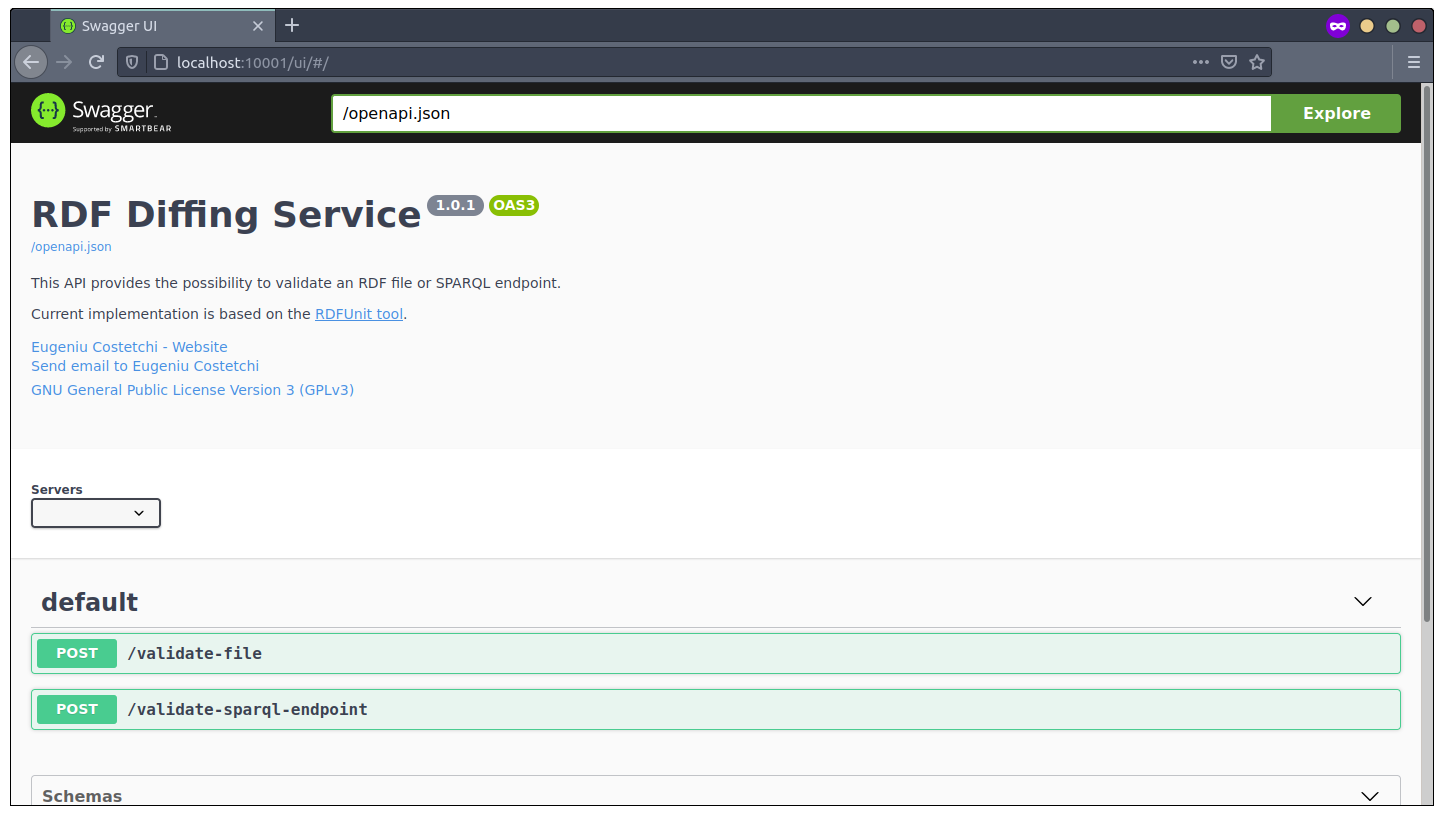
\includegraphics[width=0.9\textwidth]{images/usage/validator-api.png}
  \caption{LAM Validator API documentation}
  \label{fig:validator-api-documentation}
\end{figure} 

Here you can find the defintion for each API endpoint, the HTTP methods, request structure, and the possibility to test the endpoints.

\subsubsection{UI}
To access the user interface for the LAM Validator service visit the following link \url{http://localhost:10002}. You'll be greeted with an interface like in Figure \ref{fig:validator-ui-file} containing 2 pages.

\begin{figure}[H]
  \centering
  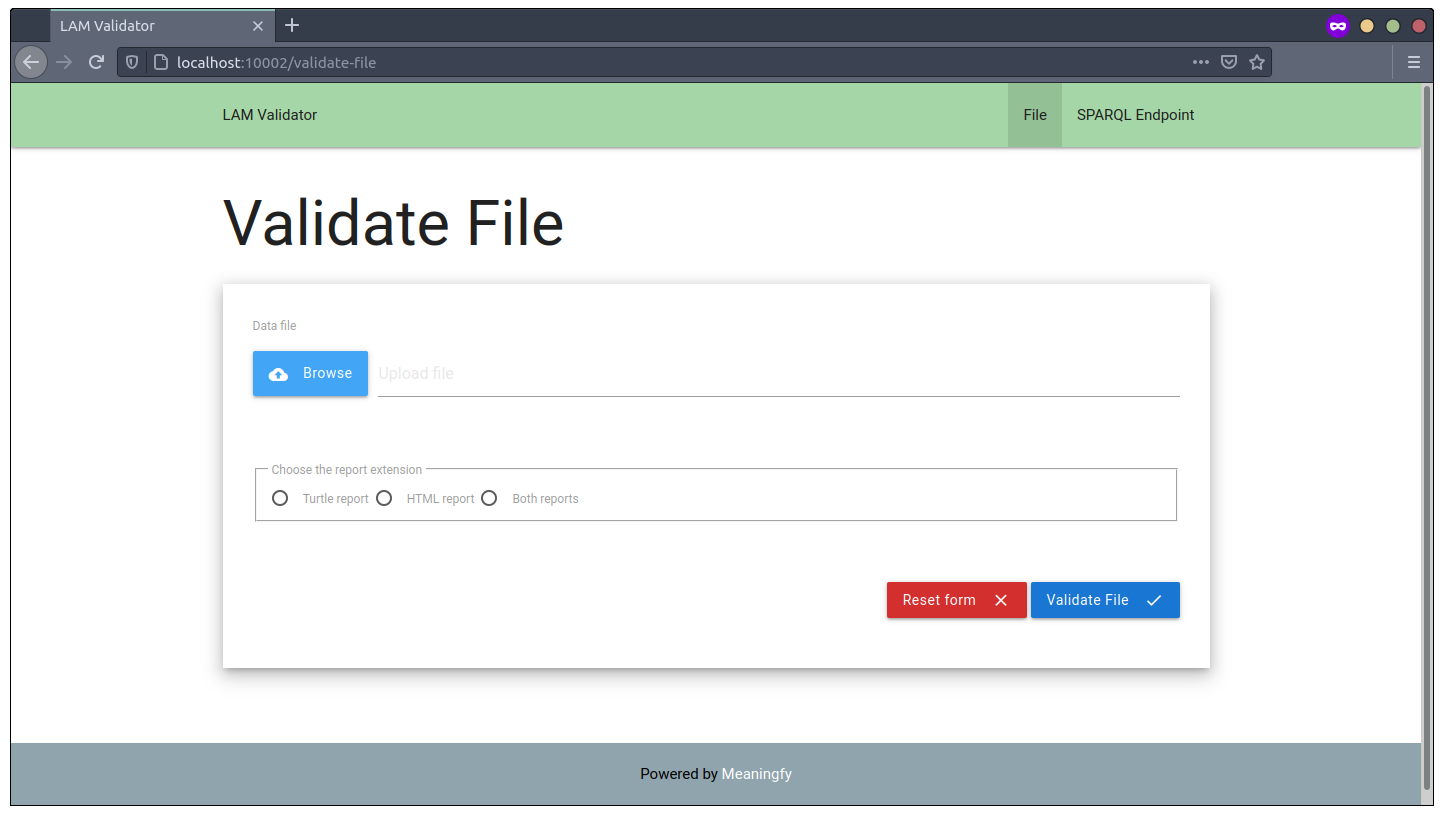
\includegraphics[width=0.9\textwidth]{images/usage/validator-ui-file.png}
  \caption{LAM File Validator UI page}
  \label{fig:validator-ui-file}
\end{figure} 

Here you can access the services for file validation (Figure \ref{fig:validator-ui-file}) and SPARQL endpoint validation (Figure \ref{fig:validator-ui-sparql}).

\begin{figure}[H]
  \centering
  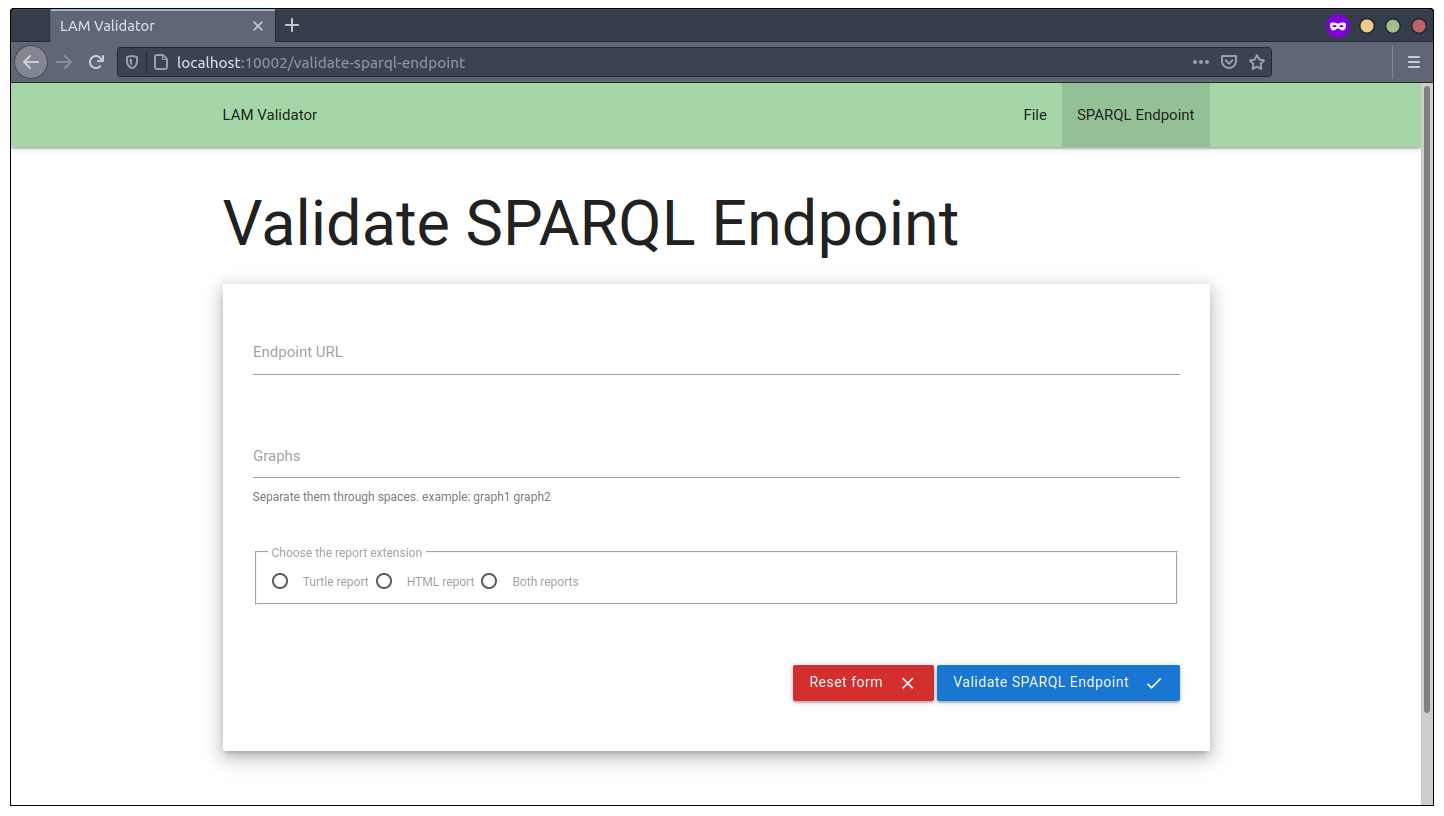
\includegraphics[width=0.9\textwidth]{images/usage/validator-ui-sparql.png}
  \caption{LAM SPARQL Endpoint Validator UI page}
  \label{fig:validator-ui-sparql}
\end{figure} 

\subsection{LAM Generation Services}
\subsubsection{API}
To access the online documentation and testing grounds for the LAM Generation Services API service visit the following link \url{http://localhost:4050/ui}. You'll be greeted with an interface like in Figure \ref{fig:lam-generation-api-documentation}.

\begin{figure}[H]
  \centering
  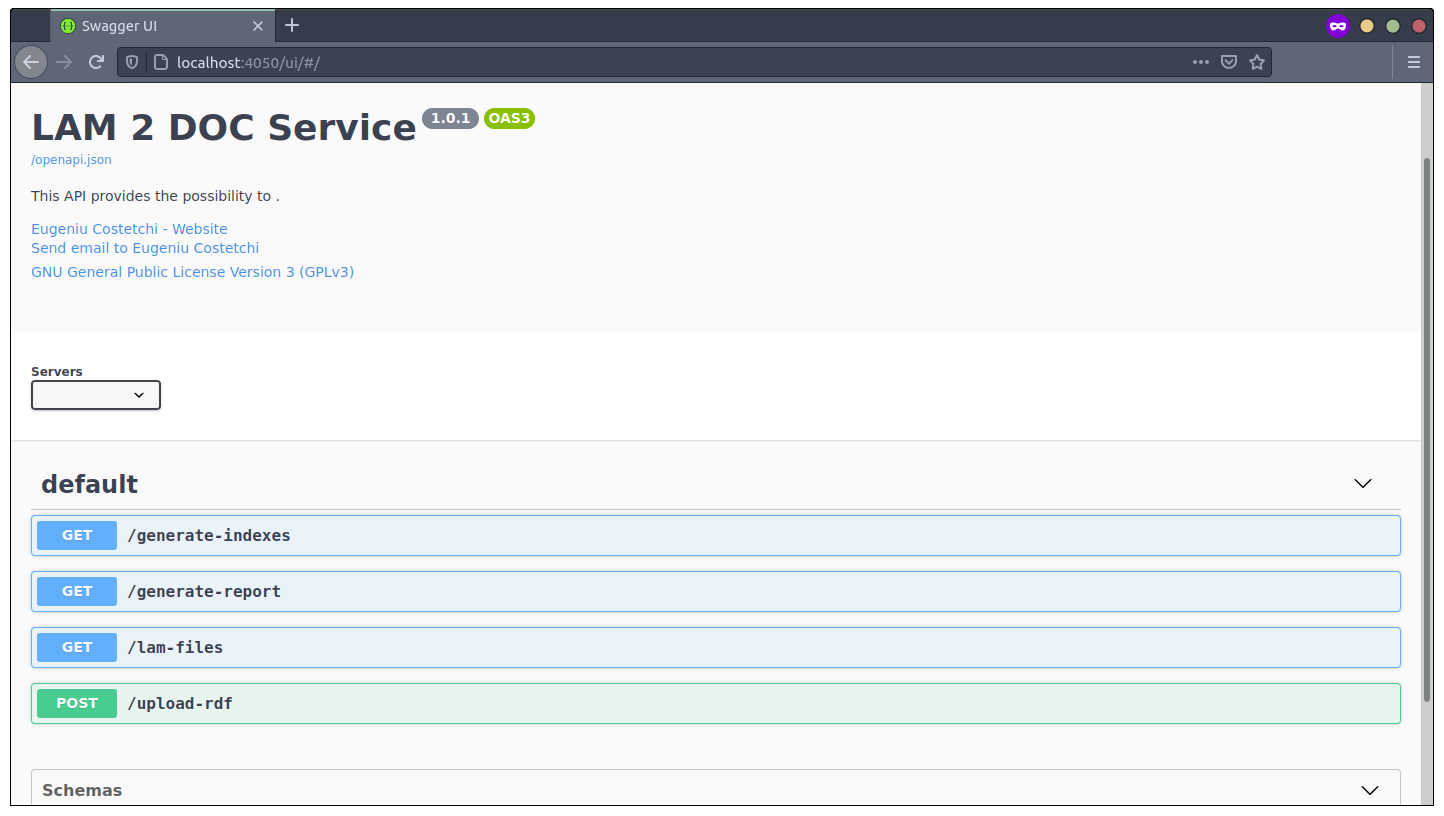
\includegraphics[width=0.9\textwidth]{images/usage/lam-generation-api.png}
  \caption{LAM Generation Services API documentation}
  \label{fig:lam-generation-api-documentation}
\end{figure} 

Here you can find the defintion for each API endpoint, the HTTP methods, request structure, and the possibility to test the endpoints.

\subsubsection{UI}
To access the user interface for the LAM Generation Services visit the following link \url{http://localhost:8050}. You'll be greeted with an interface like in Figure \ref{fig:lam-generation-ui-home} containing 2 pages.

\begin{figure}[H]
  \centering
  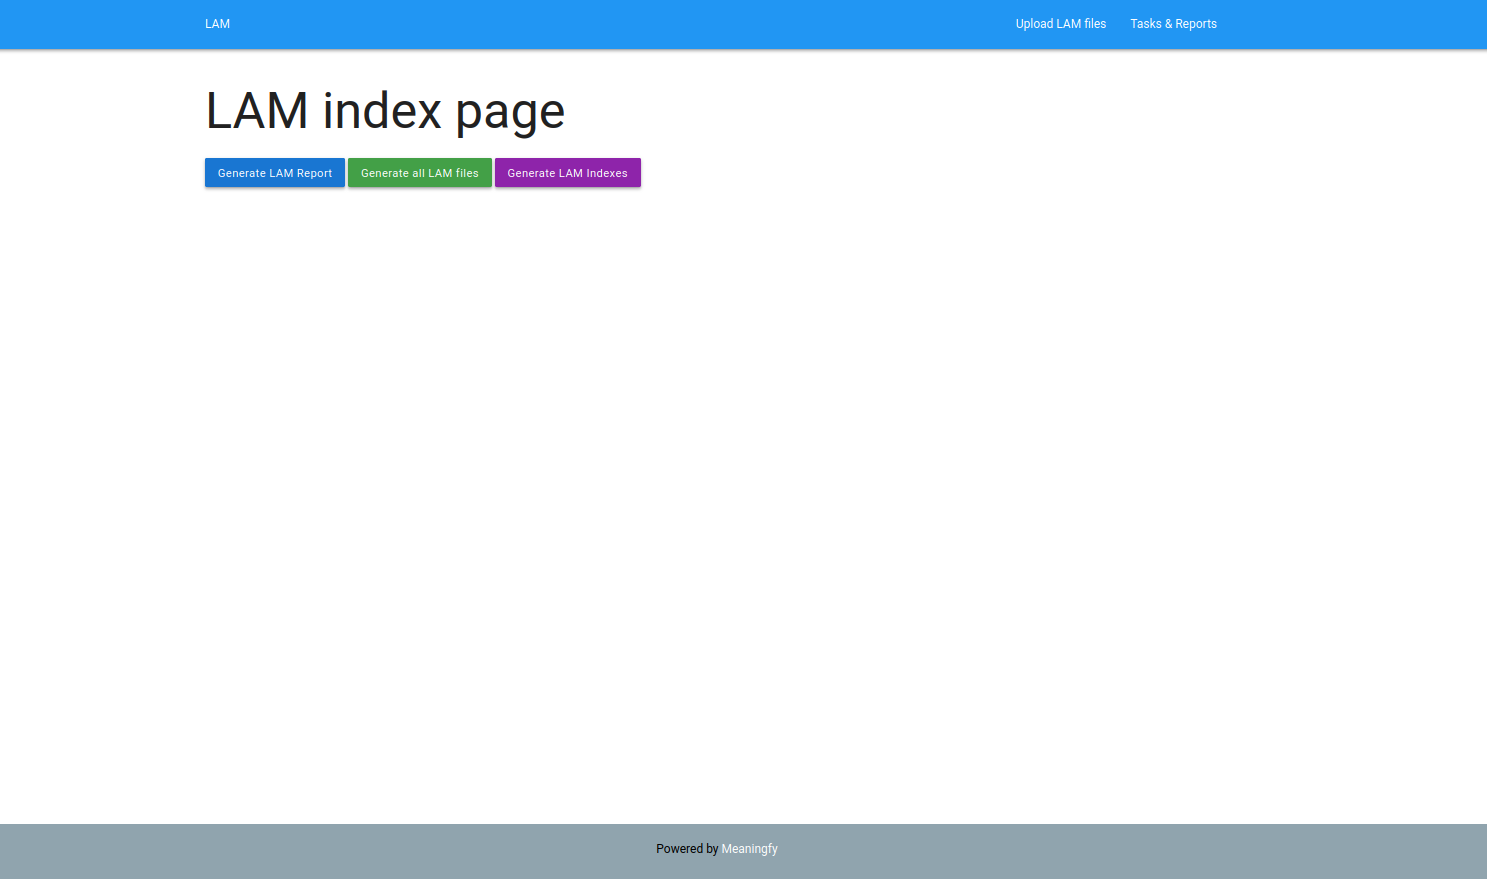
\includegraphics[width=0.9\textwidth]{images/usage/lam-generation-ui-home.png}
  \caption{LAM Generation Services home page}
  \label{fig:lam-generation-ui-home}
\end{figure} 

Here you can request the LAM report in 2 formats (Figure \ref{fig:lam-generation-ui-report}), the LAM indexes, or both report formats and indexes in a zipped format.

\begin{figure}[H]
  \centering
  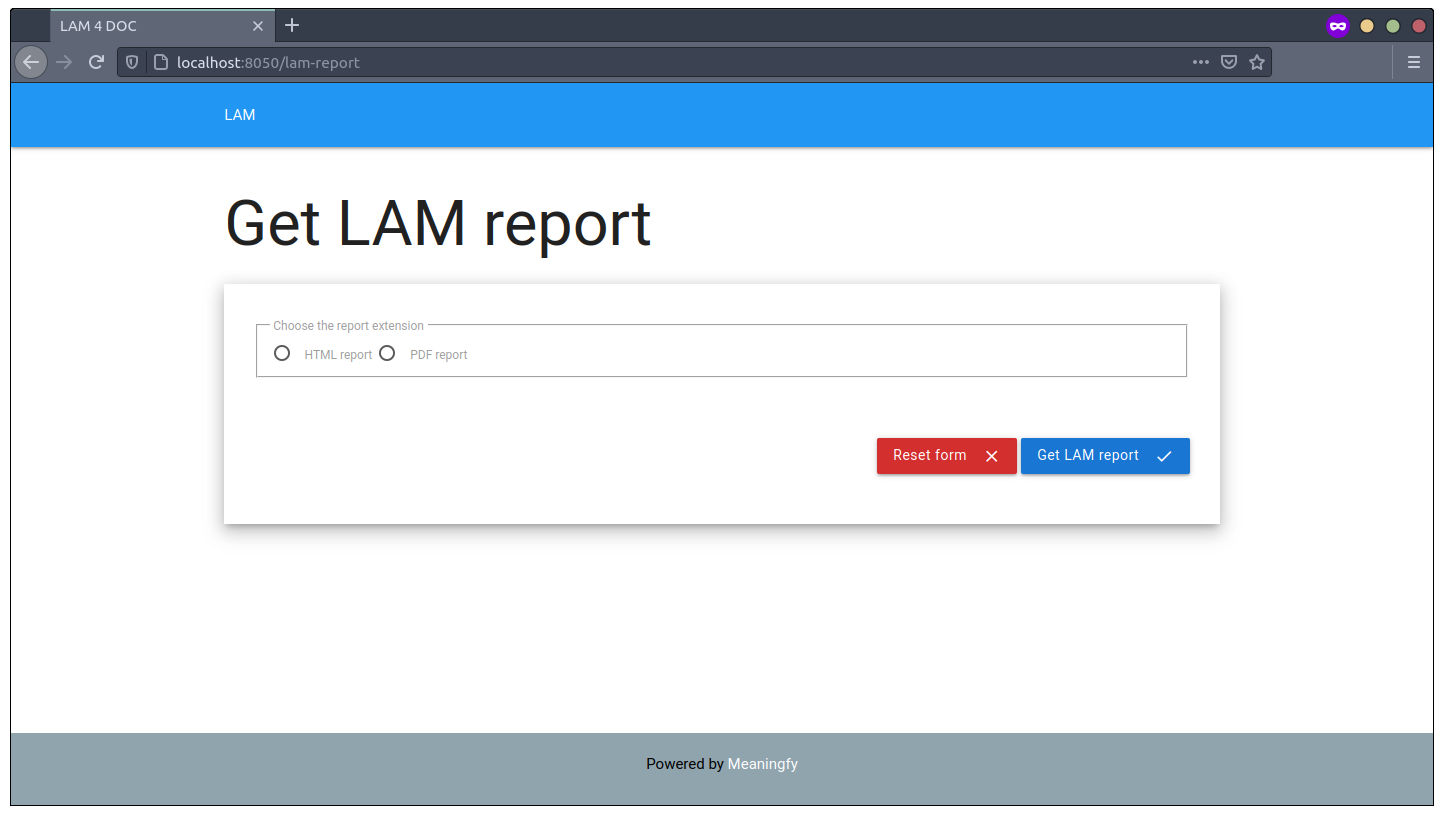
\includegraphics[width=0.9\textwidth]{images/usage/lam-generation-ui-report.png}
  \caption{LAM Generation Services report generation}
  \label{fig:lam-generation-ui-report}
\end{figure} 

\subsection{LAM Dedicated Triple Store}
To access the LAM Fuseki triple store service visit the following link \url{http://localhost:3010}. You'll be requested the login credentials which can be found in Table \ref{tab:fuseki}. After logging in, you'll be greeted with an interface like in Figure \ref{fig:lam-fuseki-home}.

\begin{figure}[H]
  \centering
  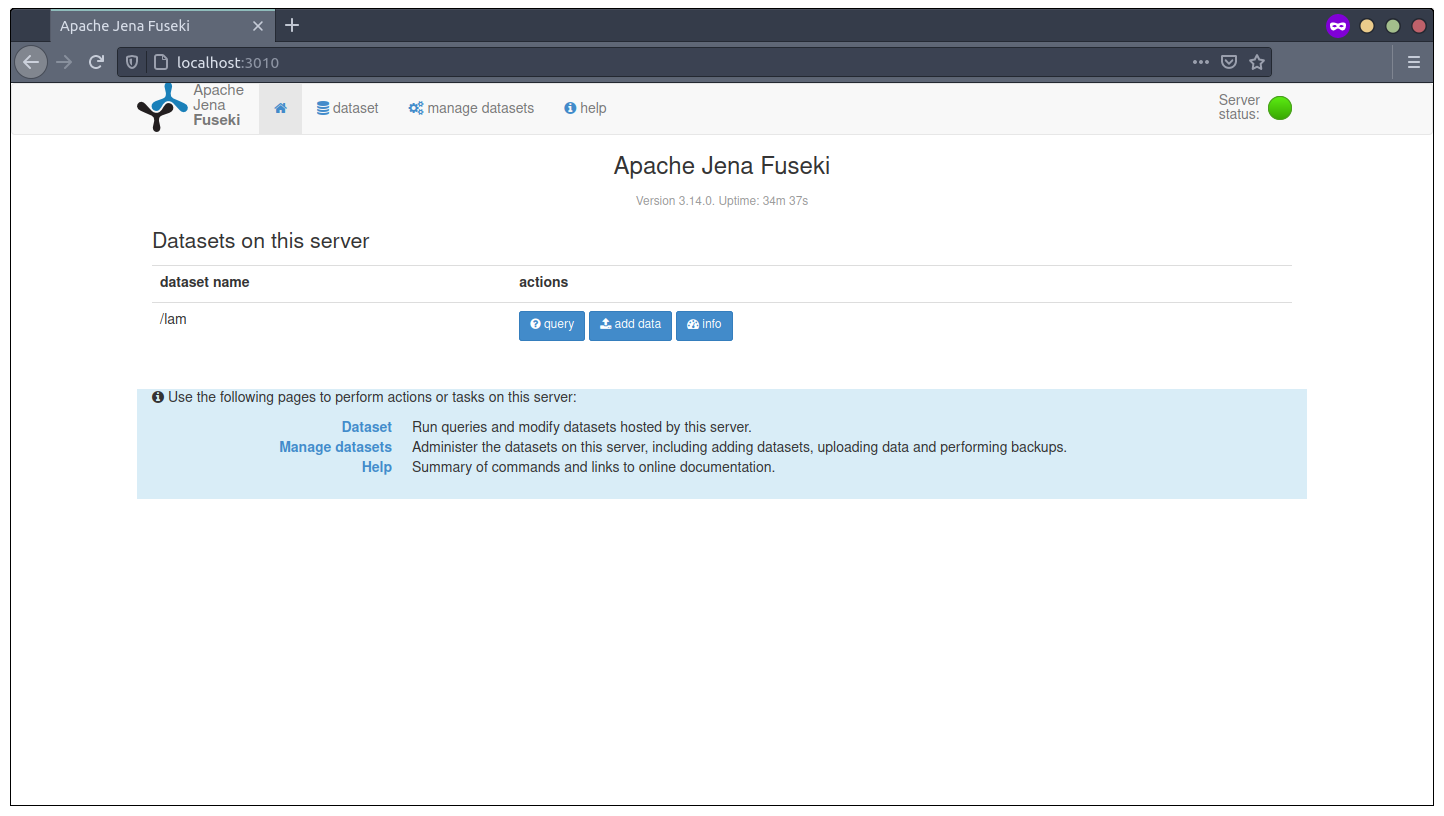
\includegraphics[width=0.9\textwidth]{images/usage/fuseki-home.png}
  \caption{LAM Fuseki home}
  \label{fig:lam-fuseki-home}
\end{figure} 

For more information on how to use Fuseki read the available documentation available at \href{https://jena.apache.org/documentation/fuseki2/}{jena.apache.org}.